\section{Auswertung}
\label{sec:Auswertung}

Zu Beginn der Messung wird die RF-Spule mit einer Frequenz von $f_{\text{HF}}=\qty{100}{\kilo\hertz}$ betrieben.
In \autoref{fig:oszilloskop} ist der Verlauf der Lichtintensität in Abhängigkeit der Magnetfeldstärke der Sweepspule
zu sehen.

\begin{figure} [H]
  \centering
  \includegraphics[height=8cm]{content/oszilloskop.jpg}
  \caption{Oszilloskopbild bei $f_{\text{HF}}=\qty{100}{\kilo\hertz}$.}
  \label{fig:oszilloskop}
\end{figure}

Auffällig sind hier die negativen Peaks der Lichtintensität, einmal bei $B=0$ und bei den beiden charakteristischen
Feldstärken der Rubidium Isotope $^{85}\symup{Rb}$ und $^{87}\symup{Rb}$.
Der Peak bei $B=0$ dient nur zu Kalibrierung und ist bei der weiteren Auswertung nicht von Interesse.

Das horizontale Magnetfeld setzt sich aus dem Feld der Sweepspule und dem Feld der anderen horizontalen Spule
zusammen. Die Felder der Spulen lassen sich direkt aus dem Strom berechnen, gemäß der Helmholtz-Gleichung:
\begin{equation}
  B =\mu_0 \frac{8NI}{\sqrt{125}R}
  \label{eq:Bfeld}
\end{equation}
Das Gesamtfeld ergibt sich aus der Summe der beiden Felder.
\begin{equation}
  B_{\text{ges}} = B_{\text{sweep}} + B_{\text{hor}}
  \notag
\end{equation}
Das Sweepfeld dient zur Variation des Magnetfeldes innerhlab eines festgelegten Bereichs, um die erwähnten Peaks auflösen zu können.
Das horizontale Feld erlaubt eine konstante Verschiebung dieses Bereiches, um die wandernden Peaks bei Erhöhung der HF-Frequenz
$f_{\text{HF}}$ im Oszilloskop verfolgen zu können.
Die Stromstärke der Sweepspule kann über die angelegte Spannung über einen Faktor von $0.1$ ermittelt werden, während die
Stromstärke der horizontalen Spule direkt gemessen wird. Die Messwerte sind im Anhang in \autoref{fig:messdaten} zu sehen.

Die HF-Frequenz $f_{\text{HF}}$ wird ausgehend von $\qty{100}{\kilo\hertz}$ in $\qty{100}{\kilo\hertz}$ Schritten erhöht,
bis eine Frequenz von $\qty{100}{\mega\hertz}$ erreicht ist.
Für jede Frequenz werden die Stromstärken der Spulen an den beiden Peaks am Oszilloskop abgelesen und anschließend wird
dann mithilfe von \eqref{eq:Bfeld} die den Peaks zugehörige Magnetfeldstärke berechnet.
Die Wertepaare für beide Isotope sind in \autoref{fig:plot} geplottet.

\begin{figure} [H]
  \centering
  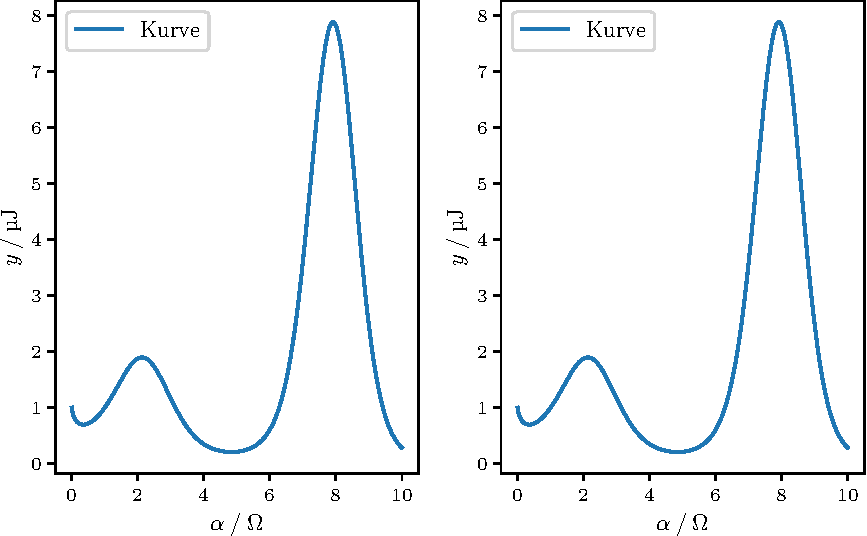
\includegraphics[height=8cm]{plot.pdf}
  \caption{Magnetfeldstärke $B$ an den Resonanzen in Abhängigkeit der RF-Frequenz $f_{\text{HF}}$, zusammen mit den zugehörigen Regressionsgraden.}
  \label{fig:plot}
\end{figure}

Fitresultat:

M1: (1.431+-0.007)e-10, B1: (2.54+-0.04)e-05
M1: (2.109+-0.019)e-10, B1: (2.64+-0.12)e-05

Erster g Faktor:0.4991+/-0.0024
Zweiter g Faktor:0.3387+/-0.0031
Erster Kernspin: I1=1.504+/-0.010
Zweiter Kernspin: I2=2.452+/-0.027